\section{Имитационное моделирование}

	В начале эксплуатации ИС <<Шерлок>> в реальных условиях обработка запросов может происходить за допустимое время, но с ростом базы знаний ИС (при каждом запросе после обработки происходит сохранение проверенной работы в БД) и числа пользователей (потонциальный функционал ИС не ограничен проверкой исходных кодов программ, и может использоваться для проверок любых типов работ, что влечёт за собой расширение круга пользователе ИС) время обработки будет увеличиваться, что может отрицательно сказаться на работе тех систем, которые взаимодействуют с ИС <<Шерлок>>.

	Для определения времени обработки работы при заданном числе запросов за единицу времени была разработана иммитационная модель в среде AnyLogic. Графическое изображение этой модели представленно на рис. \ref{img:simulation_model}.

	\begin{figure}[h]
		\center{\frame{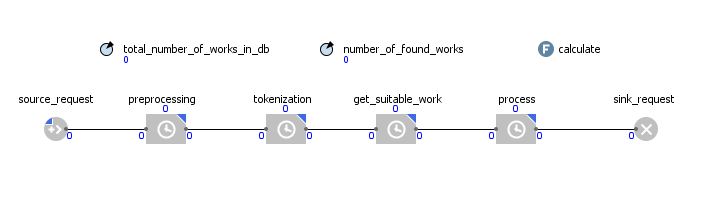
\includegraphics[width=0.8\linewidth]{simulation_model.png}}}1
		\caption{Имитационная модель обработки запроса}
		\label{img:simulation_model}
	\end{figure}

	Весь цикл обработки запроса состоит из нескольких операций, которые занимают разное количество времени:
	\begin{itemize}
		\item preprocessing - этап, на котором происходит ``очистка'' работы студента от той информации, которая ухудшает качество проверки;
		\item tokenization - этап, на котором происходит разбор исходной работы на токены, на основе которых происходит дальнейшее сравнение работ; время операции зависит от типа работы, так как обработка работ на разных языках программирования имеет различную сложность;
		\item get-suitable-work - этап, на котором происходит выборка работ из БД схожей тематики с работой, присланной на проверку;
		\item process - этап, на котором происходит сравнение найденых работ из БД с проверяемой работой; время операции зависит от числа работ, найденых для сравнения и от сложности алгоритмов, используемых при проверке.
	\end{itemize}

	В переменнах total-number-of-works-in-db и number-of-found-works хранится общее число работ в БД и число работ, найденных для сравнения с проверяемой работой соответственно.

	Время сравнения работ выисляется с помощью функции calculate. В теле этой функции считается время, затраченное на поочерёдное сравнение работ с помощью каждого алгоритма, который реализован в системе.

	Для определения конкретных значений времени обработки для каждого из этапов было произведено тестирование прототипа ИС, в результате чего были получены следующие значения:
	\begin{itemize}
		\item preprocessing - случайное значение в пределах от 10 до 20 мс;
		\item tokenization - размер проверяемой работы в байтах умноженное на случайное значение в пределах от 0,1 до 0,2 мс;
		\item get-suitable-work - общее число работ в БД умноженное на 0.0000313 мс (такое среднее время было полученно для чтения одной записи);
		\item process - сумма времени сравнения каждой найденой записи с проверяемой работой по каждому из алгоритмов.
	\end{itemize}

	После проведения тестов на разработанной модели можно определить, какой из этапов обработки является узким местом в системе. В зависимости от типа найденой проблемы можно предложить ряд мер, направленных на её устранение:
	\begin{itemize}
		\item программная реализация паралеллизма обработки запросов;
		\item уменьшение сложности применяемых алгоритмов путём применения различных эвристик;
		\item улучшение алгоритма выборки подходящих работ для сравнения.		
	\end{itemize}

